% Source: https://tex.stackexchange.com/a/656581/6880

\documentclass[border=10mm]{standalone}
\usepackage{tikz}
\usetikzlibrary{backgrounds}

\colorlet{rhombitrihexagonal tiling color one}{red}
\colorlet{rhombitrihexagonal tiling color two}{green}
\colorlet{rhombitrihexagonal tiling color three}{blue}

\begin{document}
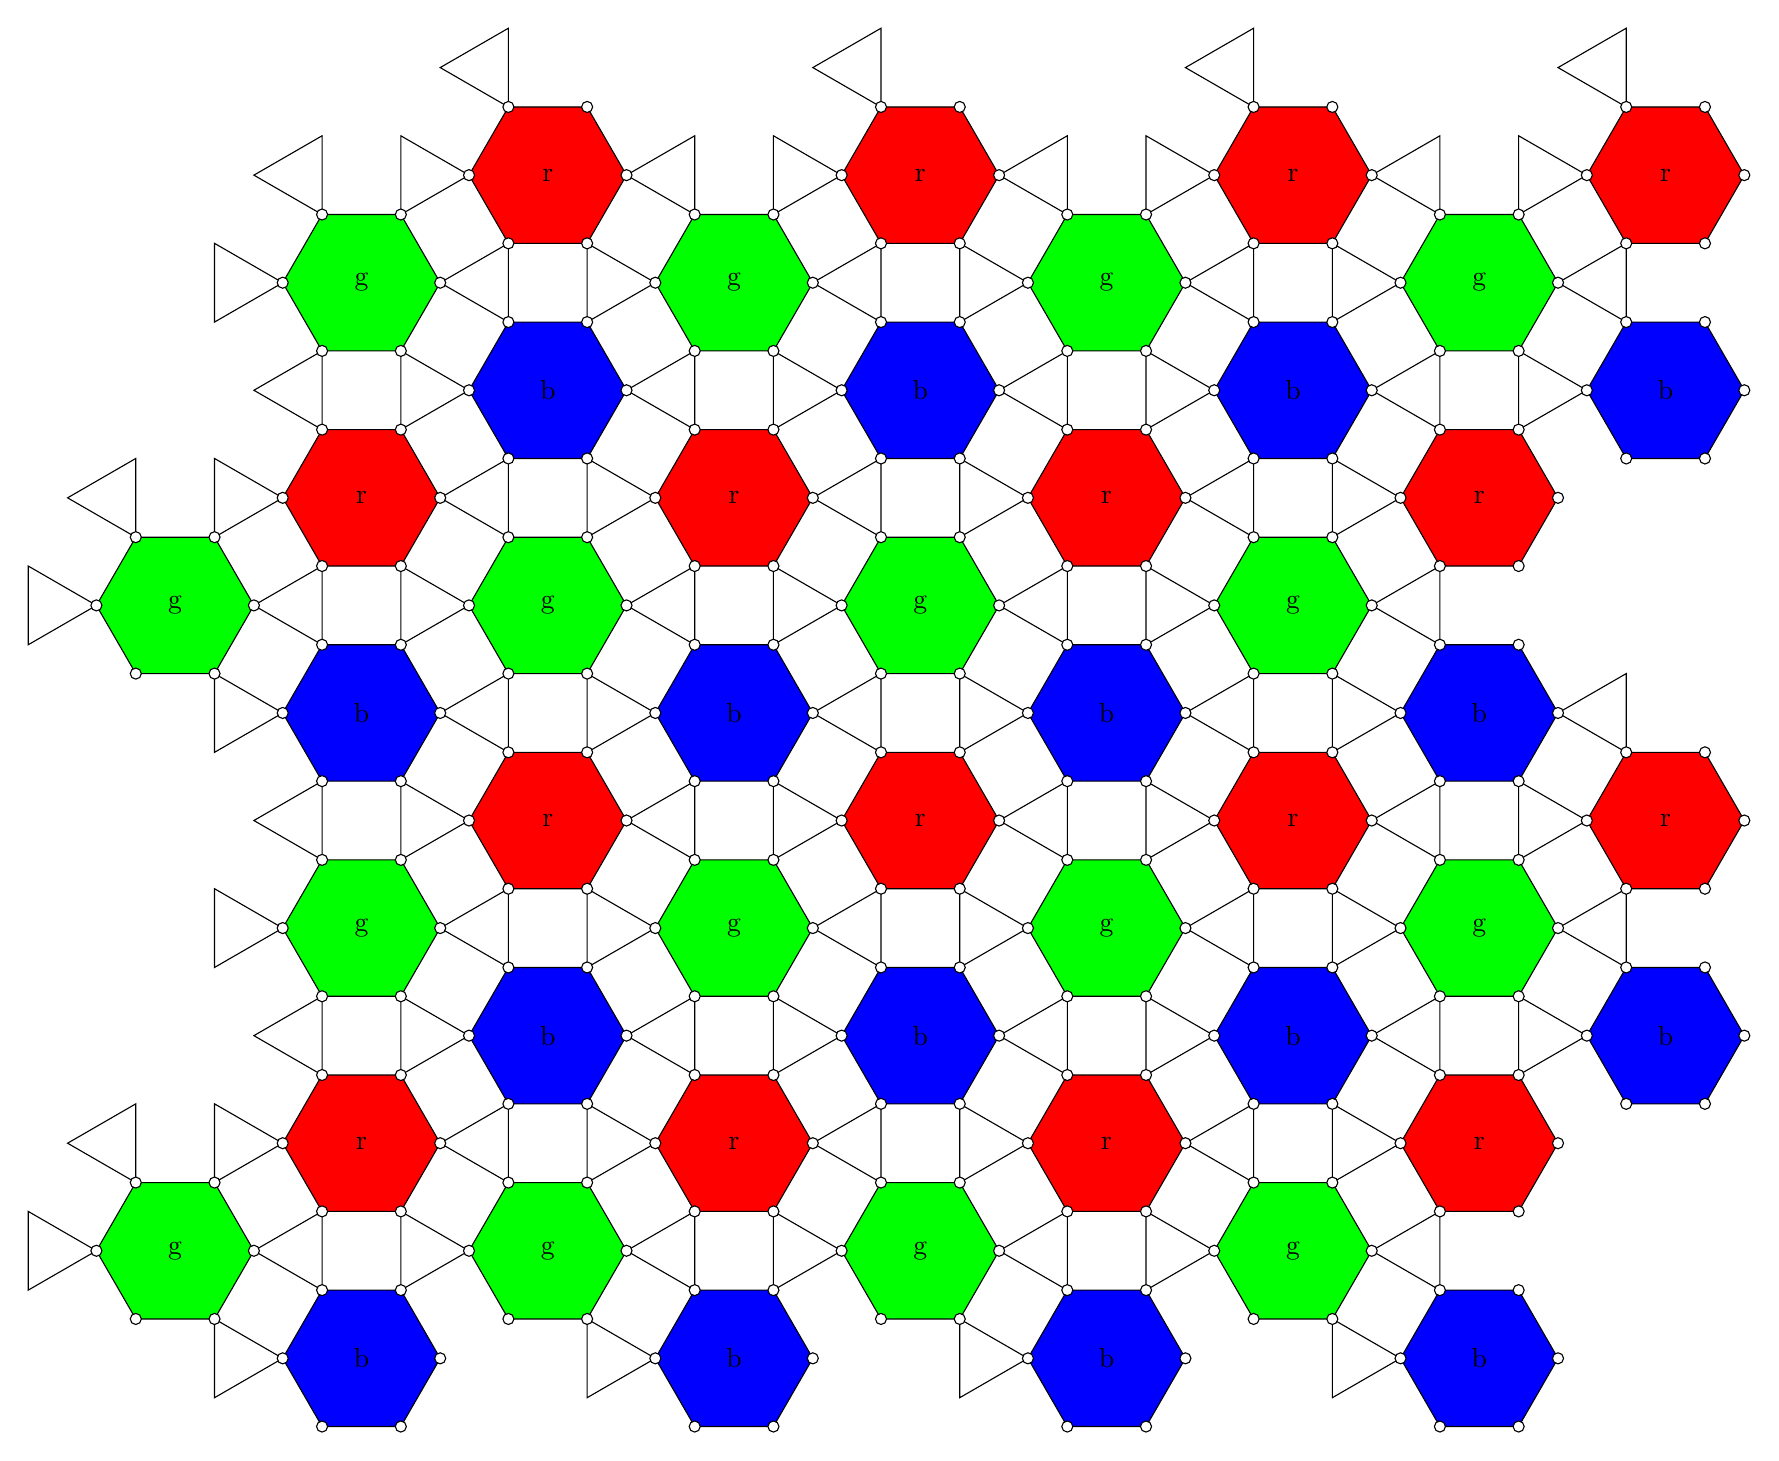
\begin{tikzpicture}[
    pics/rhombitrihexagonal tiling/.default={r}{g}{b},
    pics/rhombitrihexagonal tiling/.style n args={3}{
        code={
            \foreach \s/\c/\n in {
                (30:1+2*sin(60))/rhombitrihexagonal tiling color one/#1,
                (0:0)/rhombitrihexagonal tiling color two/#2,
                (-30:1+2*sin(60))/rhombitrihexagonal tiling color three/#3
            } {
                \begin{scope}[shift={\s}]
                    \begin{pgfonlayer}{background}
                        \draw[fill=\c] (0:1) -- (60:1) -- (120:1) -- (180:1) -- (240:1) -- (300:1) -- cycle;
                        \node at (0,0) {\n};
                        \foreach \i in {2,3} {
                            \begin{scope}[rotate=60*\i, shift={(0:1)}]
                                \draw (0:0) -- (30:1) -- (-30:1) -- cycle;
                            \end{scope}
                        }
                    \end{pgfonlayer}
                    \foreach \i in {0,...,5} {
                        \draw[fill=white] ({60*\i}:1) circle[radius=2pt];
                    }
                \end{scope}
            }
        }
    }]
  
    \foreach \y in {0,...,3} {
        \foreach \x in {0,...,3} {
            \path ({(0.5*mod(\y,2)+\x)*(3+2*sin(60))},{\y*(1.5+3*sin(60))}) pic {rhombitrihexagonal tiling};
        }
    }

\end{tikzpicture}
\end{document}
